\chapter[Research]{Research}

\section{Previous Research}
\subsection{Preconditioning}
A study done on the state of the magnetosphere for a subset of coronal mass
ejection and co-rotating interaction region events looked to identify if there
were a preconditioning under sustained northward interplanetary magnetic fields
(IMF). This paper aimed to verify a theory that a cold dense
plasma sheet prior to storm initiation, which is known to enhance the ring
current, is being caused by a sustained northward IMF. The enhancement of the
ring current would lead to lower Dst values. Measured and modeled Dst values were compared as
a validation for a semiempirical Dst model. The modeled Dst tended to
underestimate the actual measured Dst during events where there was a sustained
northward IMF before storm start. When viewing geosynchronous data from Los
Alamos, it was verified that a colder and denser plasma sheet was present for
the specified events where a sustained northward IMF was
present prior to storm initiation \cite{Lavraud2006}.

Most recently a study was done on how the ring current plays a role in steady
magnetospheric convection (SMC). SMC is a balance of reconnection rates on the
dayside and in the distant tail region. This paper believes that the ring
current strength has to be at a certain level in order for SMC to occur. Through
a study of IMF Bz and Vx along with the SYM-H index and multiple events to
examine, the research determined that most SMC events are preconditioned with
low Vx and a slightly negative Bz which would provide energy to the ring
current and prevent bursty convection from occurring allowing a continuous SMC
event \cite{Juusola2013}.
\subsection{Extreme events}
In order to better the predictability of magnetopause locations under extreme
events, \cite{Shue1998} Shue took satellite measurements where there were
magnetopause crossings and compared them to two models. The first model
(Petrinic and Russell 1996) was compared to his model (Shue et. al. 1997). Both
models did quite well with magnetopause crossings at the dayside magnetopause,
while the Shue model had a tougher time with magnetopause crossings at the
flanks. The determination for the disrepencies were ``due to the
inappropriate linear extrapolation from the parameter range for average
solar wind conditions to that for extreme conditions''. Upon fixing the errors
the Shue model was able to better predict the magnetopause flank crossings.

Companies that operate in space are very interested in the longevity of extreme
storms. A paper by Cid et. al. \cite{Cid2013} researches the effectiveness of
using a hyperbolic function to estimate the decay time after an extreme storms
peak Dst values. They use the work of previous research in where a linear function was
used to estimate the decay time for non-extreme events. The reason they use a
hyperbolic function was because a linear function did not work well for the
decay time of extreme storms. The extremity of the storm was determined by the
Dst index where data was available, and a ``Local Disturbance Index'' taken from
the H component of geomagnetic field measured at each local observatory where
Dst data was not available.

Not all extreme events in the magnetosphere are looked at by a physics model.
A statistical analysis on the long range correlations was done in a paper by
Sharma and Veeramani \cite{Sharma2011} that uses a database of over 5 million
events. The basis for the research was that dynamical and statistical features
in extreme events are complicated due to the turbulent nature of the solar wind.
An auto-correlation function and a detrended fluctuation analysis were done to
find the long range correlations.
\subsection{Model output difference imaging}

\section{Why do a Verification and Validation study?}
V\&V is an ongoing process. What the space weather community has accepted today
as acceptable V\&V practices may slowly go out of date as science and human
capabilities proceed forward. Bringing new ideas and methods of V\&V forward and
using them to bring a different viewpoint to the scientific community is beneficial
whether it is a major success or not. New V\&V tools are vital to improving
space weather models, in turn providing space weather forecasters with better
knowledge of models and which to use for the best guidance. In this
research, a new idea will be described and then used to answer a few space
weather problems. This will provide a different view on the performance of
models to specific types of input parameters. Two of the validation
techniques described by Sargent \cite{Sargent2004}, comparison to other models,
and parameter variability will be used to answer the space weather questions
that follow.
\subsection{Preconditioning}
The preconditioning described in the paper by Lavraud \cite{Lavraud2006} uses
the term preconditioning to describe the condition of the magnetosphere thought
to cause lower Dst values in certain storms.
The preconditioning described in the paper by Juusola \cite{Juusola2013} uses
the term preconditioning as a set of specific conditions that must be met in
order to SMC events to occur.
The term preconditioning used in these papers is used to mean an actual state
that the magnetosphere needs to be in for a certain output to happen. The
preconditioning that this research is looking into is that in which takes place
in models before specific event conditions start. Magnetospheric models are
started with initial conditions and then run for a certain amount of time from
those initial conditions to the parameters set to start the run so that the
magnetosphere can remain stable. What lacks any research is the time that is
typically taken to get a stable magnetosphere, which is what this specific
section looks into more.
\subsection{Extreme events}
In the paper by Shue \cite{Shue1998}, the extreme events were past events that
had taken place and the results were specific to the events looked at.
Forecasters gain only small ground in this case into understanding the best
model to use for a certain future event.
In the paper by Cid \cite{Cid2013}, the extreme events were also past events
that had taken place where the research was looking into a better way to predict
a broader range of extreme events. There were a limited number of events looked
at, and the model used (a hyperbolic fit) was only one.
In the paper by Sharma \cite{Sharma2011}, the extreme events studied were ones
compiled from a database. Even though the use of the data was not model
based and focused on the statistics, it was still lacking comparison to other approaches.
By looking into multiple models given the same generic input, along with the
extremes of input variables, we're allowing forecasters to have a better idea of
which model is best to use for a variety of futuristic space weather events.
\subsection{Model output difference imaging}

\section{Methodology}
Two new space weather validation tools will be used to solve a few space
weather questions. The first tool is a form of the validation technique
described by Sargent called comparison to other models which will be called model
output difference imaging. This tool can be used on three dimensional data sets to
visualize the differences between two models in one plot. The second tool is a
form of the validation technique described by Sargent called parameter
variability \cite{Sargent2004}. This parameter variability technique is used by
inserting physically significant data into magnetospheric MHD models that are
not in-situ based in order to inspect the model outputs. All of the data input
into the chosen models will be done using this technique.
This new technique is applicable to any space weather model. The focus of this
research is on magnetospheric models. There are many types of magnetospheric
models, and the time required to make a comparison between them all would be
enormous. It is this reason that MHD magnetospheric models were chosen.
The computational and time requirements required to implement magnetospheric MHD
models individually as a part of this research would be costly. To satisfy the
limits of implementing the model locally, the choice to use the community
coordinated modeling center (CCMC) was made. The CCMC offers public availability
to create personalized space weather model runs as well as the availability to
obtain the results. The CCMC provides numerous space weather models, and a
subset of those models are focused on the magnetosphere \cite{CCMCModels}. The
model choice is limited further by the limits of open source software available
from the CCMC used to interpolate data, which will be described later.

\subsection{Acquiring Data}
The uniqueness to the parameter variability tool described previously is that
the data will not be input into the models as in-situ measurements from the
past, but as constant yet physically significant data taken from in-situ
measurements that have no relation to a specific previous event, but still has
meaning to the space weather community.
The CCMC allows for model runs to be created through an online web form that is
submitted to staff who will then process the submitted model runs. The input
parameters are submitted through a data file that contains data for B(x,y,z),
V(x,y,z), rho, T, or a specific event time can be specified and data will be
downloaded and used in the submitted model run.  All of this data is available
to the space weather community and was measured from the Advanced Composition
Explorer (ACE) spacecraft which sits at the L1 point ahead of the Earth in the
Sun to Earth line. The importance of this point is that the orbit and distance
from the Sun and the Earth allows for the satellite to sit in front of Earth's
orbit at all times. The ACE data was gathered from the OMNIWeb web site provided
by the NASA Goddard Space Flight Center \cite{OMNIWeb} between the dates of
January 1st, 2000 to January 1st, 2011. This contains the number of years in
the average solar cycle of 11. The data set had missing data points that needed to
be accounted for. Table \ref{table:MissingData} shows what the missing data was
represented as in the ACE data files.

\begin{table}
\begin{center}
  \caption{How missing values are represented in ACE data output}
  \begin{tabular}{| c | c | }
    \hline
    \textbf{Variable} & \textbf{Missing Data Label} \\ \hline
    n & 999.9  \\ \hline
    T & 9999999  \\ \hline
    B(x,y,z) & 999.9 \\ \hline
    V(x,y,z) & 9999 \\ \hline
  \end{tabular}
  \label{table:MissingData}
\end{center}
\end{table}

\begin{figure}
	\centering
	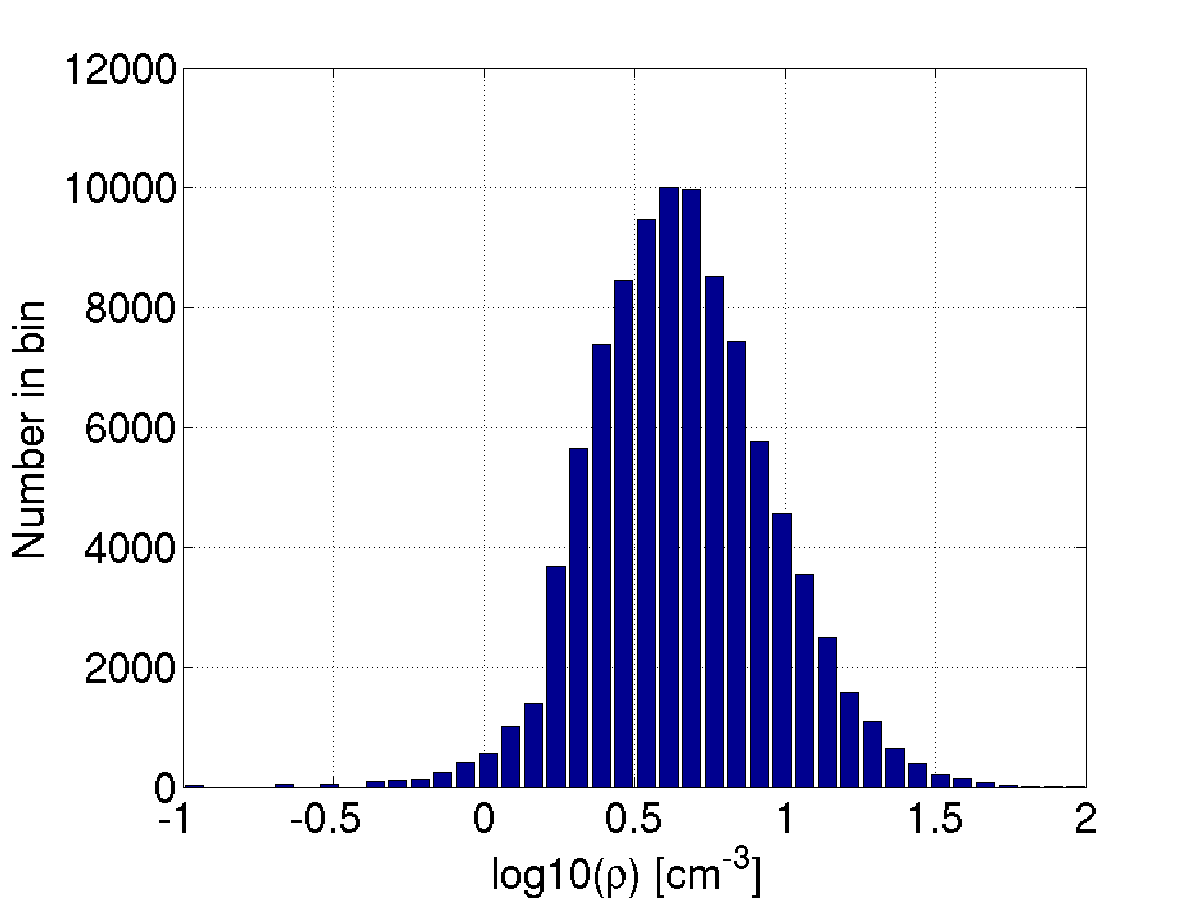
\includegraphics[scale=0.5]{images/hist_N.png}
	\caption{Histogram of solar wind density values from January 1st, 2000 to
	January 1st, 2011}
    \label{fig:hist_n}
	\figSpace
\end{figure}
\begin{figure}
	\centering
	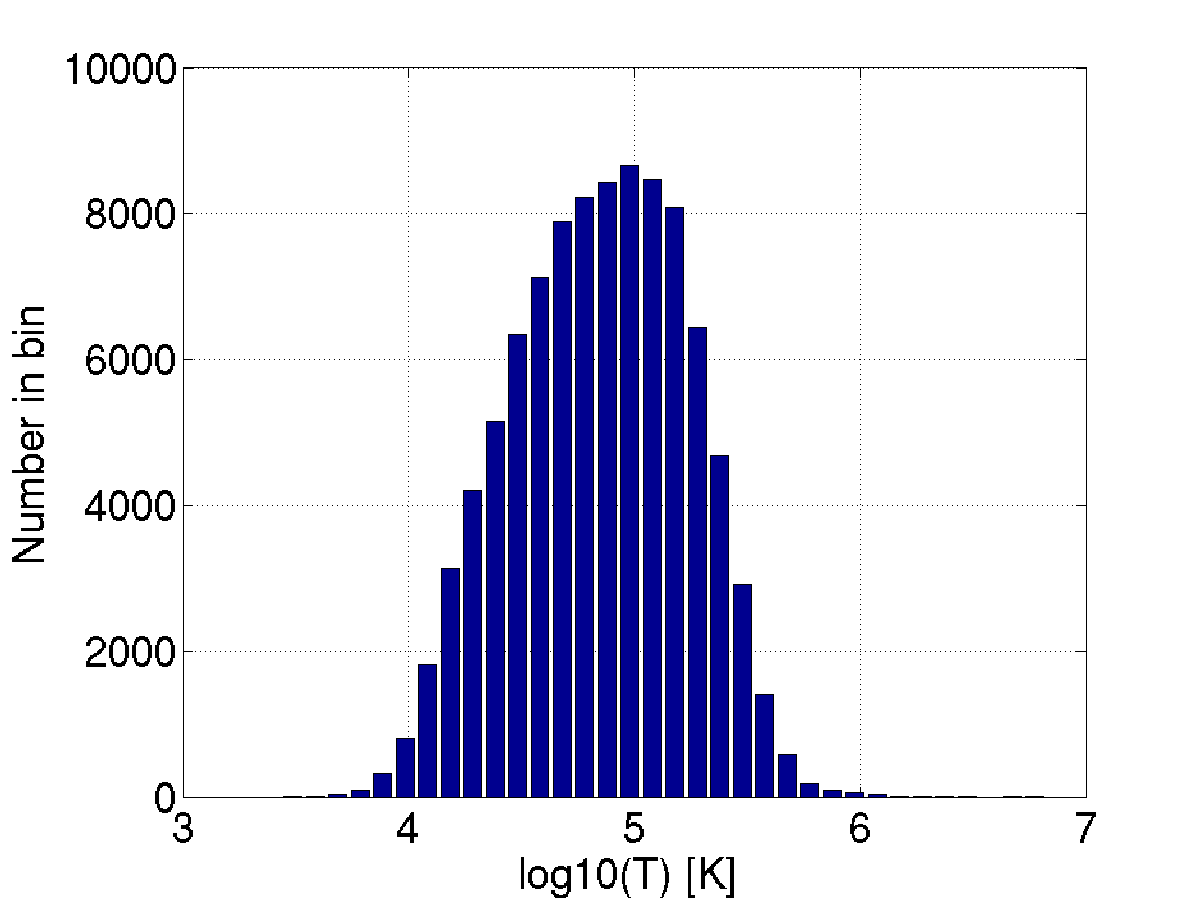
\includegraphics[scale=0.5]{images/hist_T.png}
	\caption{Histogram of solar wind temperature values from January 1st, 2000 to
	January 1st, 2011}
    \label{fig:hist_t}
	\figSpace
\end{figure}
\begin{figure}
	\centering
	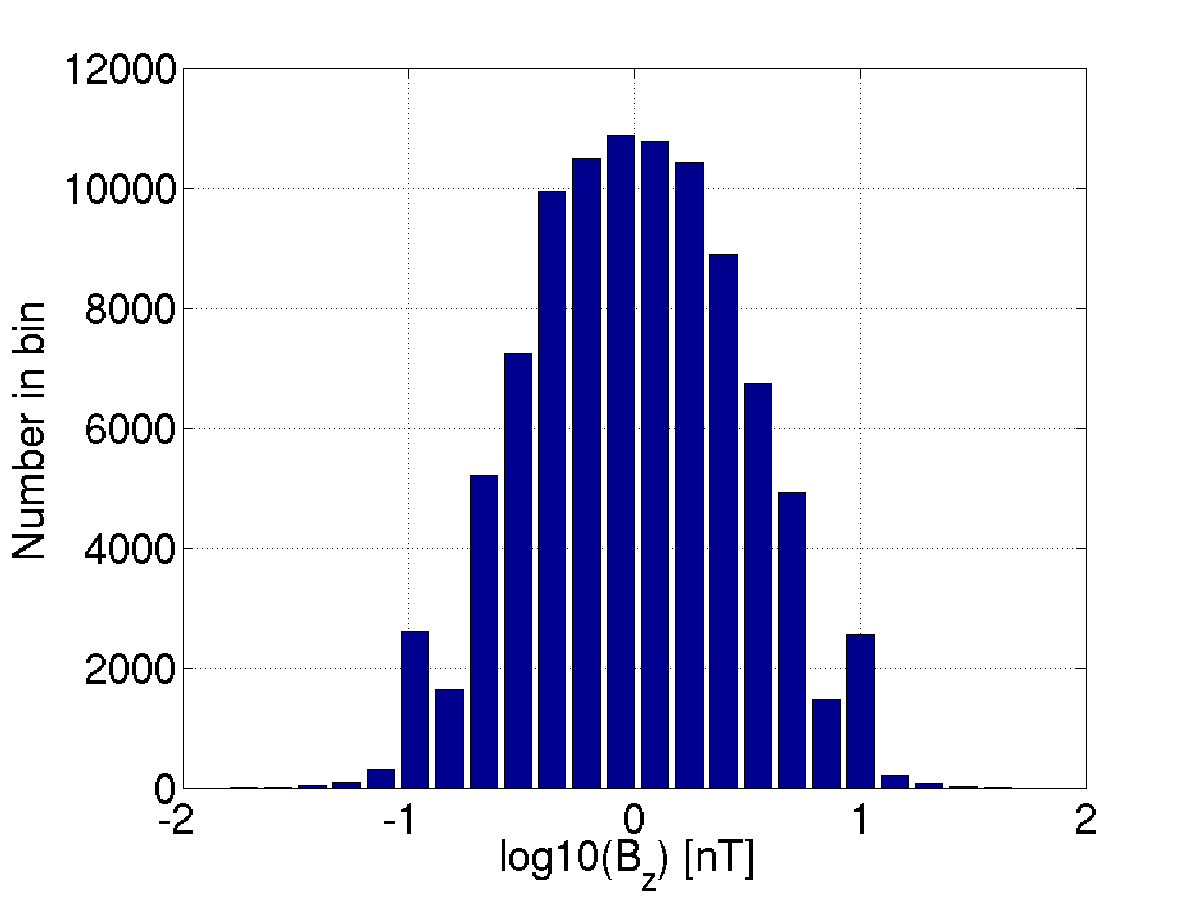
\includegraphics[scale=0.5]{images/hist_BZ.png}
	\caption{Histogram of solar wind interplanetary magnetic field strength
	(z-component) values from January 1st, 2000 to January 1st, 2011}
    \label{fig:hist_bz}
	\figSpace
\end{figure}
\begin{figure}
	\centering
	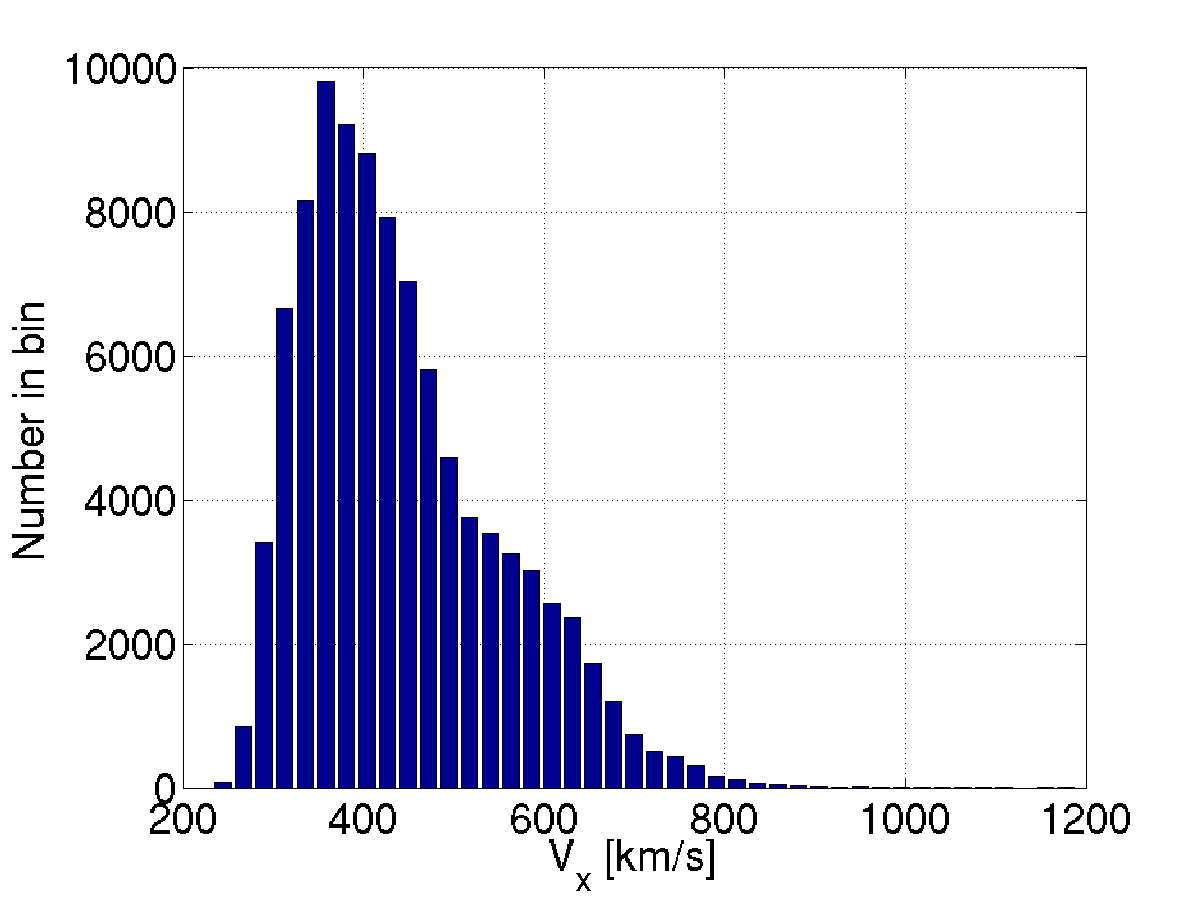
\includegraphics[scale=0.5]{images/hist_V.png}
	\caption{Histogram of solar wind velocity values from January 1st, 2000 to
	January 1st, 2011}
    \label{fig:hist_v}
	\figSpace
\end{figure}

Once the data was acquired and understood, we then used MATLAB software to read
in the data, which was in common data format (.cdf), and plotted histograms for
the variables required for input into the CCMC forms. Image \ref{fig:hist_n} is
the histogram of solar wind plasma density in number per cubic centimeter
[$cm^{-3}$]. The mean is 5.76 [$cm^{-3}$], the 90th percentile is 11 [$cm^{-3}$]
and the 10th percentile is 2 [$cm^{-3}$]. Image \ref{fig:hist_t} is the
histogram of solar wind temperature in Kelvin [$K$]. The mean is 101288.59
[$K$], the 90th percentile is 217139 [$K$] and the 10th percentile is 20554
[$K$].
Image \ref{fig:hist_bz} is the histogram of the solar wind interplanetary magnetic
field in nanotesla [$nT$]. The mean is 0.02 [$nT$], the 90th percentile is 3.1
[$nT$] and the 10th percentile is -3.0 [$nT$]. Image \ref{fig:hist_v} is the
histogram of solar wind velocity in the x direction in kilometers per second
[$Km/s$]. The mean is 441.710 [$Km/s$], the 90th percentile is 604 [$Km/s$] and
the 10th percentile is 310 [$Km/s$]. The reasons for the choices of the 10th and
90th percentile will be described later. The values for each variable are
displayed in Table \ref{table:histtable}.

\begin{table}
\begin{center}
  \caption{ACE solar wind data histograms mean, 10th and 90th percentiles}
  \begin{tabular}{| l | c | c | c | }
    \hline
    \textbf{Variable} & \textbf{10th Percentile} & \textbf{Mean} &
    \textbf{90th Percentile} \\
    \hline n & 2 & 5.76  & 11   \\ \hline
    T & 20554 & 101288.59  & 217139 \\ \hline
    Bz & -3.0 & 0.02 & 3.1 \\ \hline
    Vx & 310 & 441.710 & 604 \\ \hline
  \end{tabular}
  \label{table:histtable}
\end{center}
\end{table}

To demonstrate the use of the tools previously mentioned, a few space weather
questions are presented and answered. First, to demonstrate the usability of a
code to difference the results from two model outputs as well as a parameter
variability validation, a question was posed on the preconditioning of
magnetospheric MHD models.
\subsection{Preconditioning}
According to Raeder \cite{Raeder2003} and Buchner \cite{Buchner2003}, the
magnetosphere will form within one hour from start of preconditioning. The setup
to start the preconditioning in magnetospheric models are first to set a dipole
at the position of the Earth and one sunward in order to create a region in the
magnetosphere where B=0 sunward of the Earth. The sunward dipole is then removed
and the preconditioning is started. Buchner presents a question to the community
when discussing the length of preconditioning time used in magnetospheric MHD
models. He mentions that since the magnetosphere has a long memory from previous
conditions that it may take a few hours of preconditioning time to stabilize the
magnetosphere before the initial conditions are inserted, but to this point
there has been no time put towards an answer to that question.
The key to parameter variability is that only slight changes are made to the
input conditions in order to keep as much variables constant as possible.
Deciding to use the CCMC models for this research, only changing the input
parameters into the models allows for all else to stay as close to
constant as possible.

\begin{figure}
	\centering
	\subfloat[Run 1\label{fig:run1}]{%
      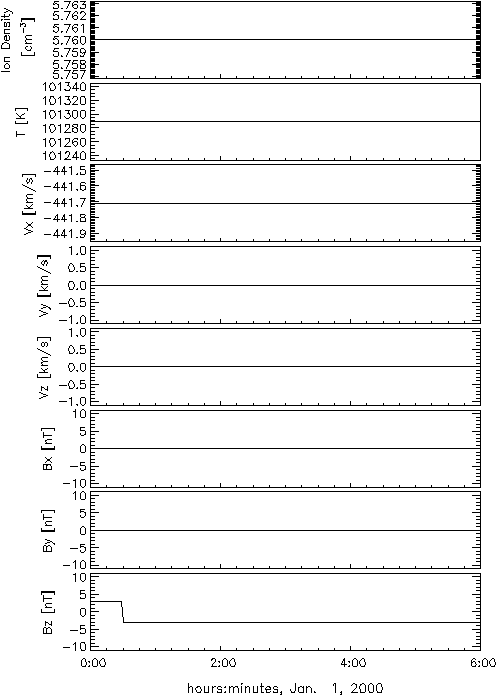
\includegraphics[width=0.45\textwidth]{images/Run1.png}
    }
    \subfloat[Run 2\label{fig:run2}]{%
      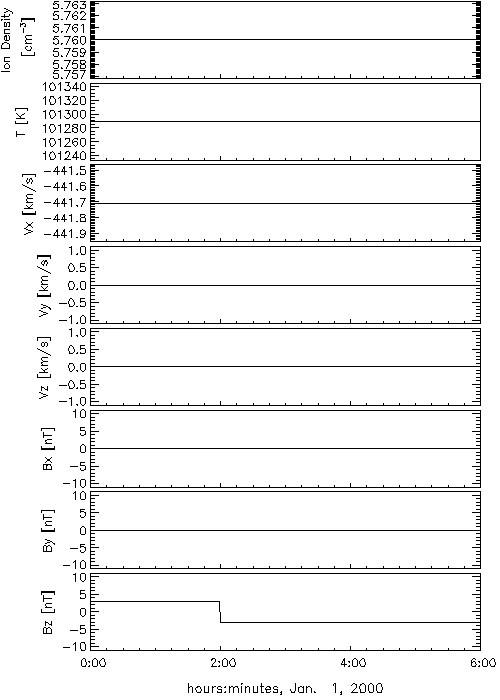
\includegraphics[width=0.45\textwidth]{images/Run2.png}
    }
	\caption{CCMC run submissions to answer preconditioning question.}
	\label{fig:preconditioning}
	\figSpace
\end{figure}

The difficulty in using the CCMC to experiment with the preconditioning time is
that the ability to change the amount of time set to precondition each MHD model
run from the web form was not available. In order to simulate the extension of
preconditioning time, it was decided to move the time for a flip in Bz to a
later time in the run and compare the models output before, during, and after the
flip, which is shown in Figure \ref{fig:preconditioning}. In order to get the
best comparison, the usage of the three dimensional differencing tool will be used.

\begin{table}
\begin{center}
  \caption{Chosen values for CCMC runs}
  \begin{tabular}{| l | c | c | c | c | }
    \hline
    \textbf{Run Num.} & \textbf{$\rho$} & \textbf{$T$} & \textbf{$Vx$} &
    \textbf{$Bz$}
    \\
    \hline 
    1 & 5.76 & 101289 & -441.71  & +3.1 to -3.0 at 00:30 \\ \hline
    2 & 5.76 & 101289 & -441.71  & +3.1 to -3.0 at 02:00 \\ \hline
    3 & 11 & 101289 & -604 & -3 \\ \hline
    4 & 2 & 101289 & -320 & 3.1 \\ \hline
  \end{tabular}
  \label{table:runs}
\end{center}
\end{table}

As shown in Table \ref{table:runs} and in Figure \ref{fig:preconditioning} for
run one, to simulate the extension of model preconditioning, we kept T, Vx, and
$\rho$ at mean values and constant throughout the entire run. The only
difference between the two runs was the time that Bz was flipped, or changed
from a positive to negative value. This is physically meaningful as a Bz flip is
a typical cause for stormy conditions in the magnetosphere.

\subsection{Extreme events}

\begin{figure}
	\centering
	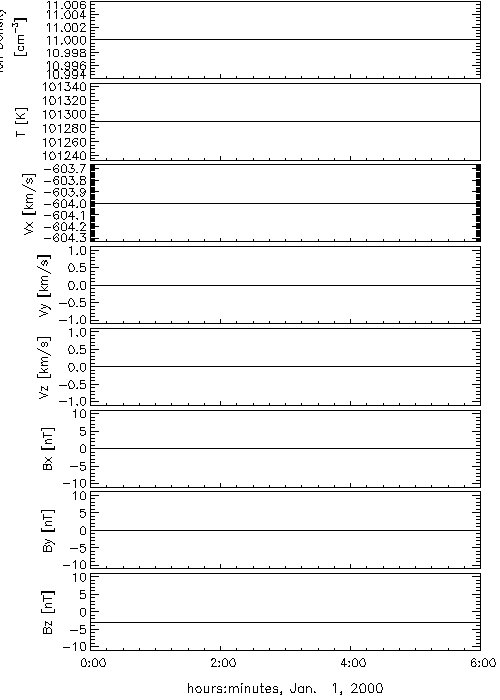
\includegraphics[scale=0.5]{images/Run3.png}
	\caption{Run for high compression event.}
    \label{fig:highcompression}
	\figSpace
\end{figure}

As shown in Table \ref{table:runs} and in Figure \ref{fig:highcompression}, in
order to compress the magnetosphere we have chosen a high solar wind velocity a
negative solar wind magnetic field and a high solar wind density. With a high
compression, magnetospheric features may be hard to resolve based on the models
resolution not being fine enough. This is physically meaningful because with
high compression there's a potential risk that the magnetopause will cross
inside geosynchronous orbit which may pose major problems for space operations.

\begin{figure}
	\centering
	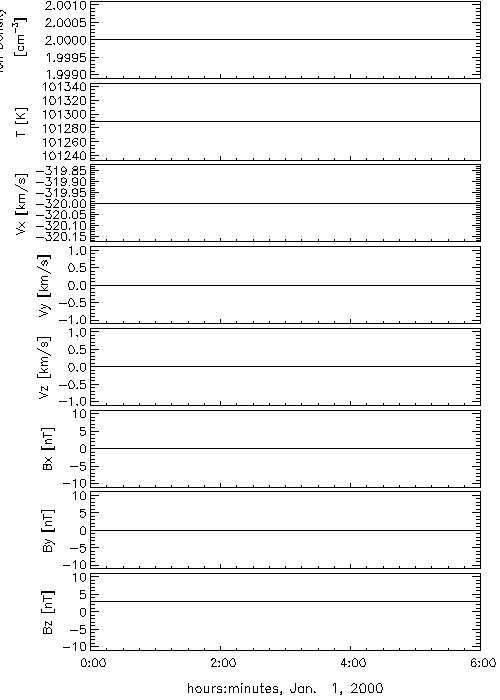
\includegraphics[scale=0.5]{images/Run4.png}
	\caption{Run for low compression event.}
    \label{fig:lowcompression}
	\figSpace
\end{figure}

For a low compression, shown in Table \ref{table:runs} and in Figure
\ref{fig:lowcompression}, we have chosen input variables that will minimize the
compression of the magnetosphere in a low solar wind velocity, a positive Bz and
a low density. With a low compression, magnetospheric features may be easier to
resolve as the resolution of the models would be finer than needed.

\subsection{Model output difference imaging}
As previously mentioned, one of the tools that will be used is a three
dimensional model output difference image. When comparing two models through
visual inspection of each output separately there is a large difficulty involved
in determining what the major differences between the two are. The support for
developing a three dimensional model output differencing code was to make that
type of comparison much easier and quicker to do. What first needed to be done
was to find a way in which to encompass all the different domains in each of the
MHD magnetospheric models into one and to have the ability to interpolate all
the different scalars in all the different MHD magnetospheric models onto the
newly created magnetospheric domain. There is one open source tool created by
the CCMC that will allow both of these to be done in the same code base. This
tool is called Kameleon \cite{Kameleon}. Kameleon is a C++ based code that
supports a few of the available CCMC MHD magnetospheric models in interpolation
of scalar outputs. It is this final limitation that determines out model output
choice for each of the experiments listed above. The Kameleon software supports
the OpenGGCM, BATS-R-US, and SWMF, and these three MHD magnetospheric models are
used to solve the questions posed in this research. Finally a tool was needed
that would be able to load such a large data set, be able to plot all of the
data, and also have the ability to take planar cuts of the data for easy
visualization. Another open source tool available to the public is called
Paraview \cite{Paraview} and is maintained by Kitware. Paraview is software that
was specifically made to visualize scientific data that can handle very large data
sets and offer an availability to parallelize operations so that plotting may go
faster. There are many plotting tools available which includes the ability to
visualize a slice of a larger data set. Paraview also offers python code support
that allows for plots to be made automatically instead of using their
sophisticated graphical user interface.
